\documentclass[aps,pra,twocolumn,amsmath,amssymb,nofootinbib,superscriptaddress]{revtex4}

\newcommand{\bra}[1]{\langle#1|}
\newcommand{\ket}[1]{|#1\rangle}
\newcommand{\op}[2]{\hat{\textbf{#1}}_{#2}}
\newcommand{\dagop}[2]{\hat{\textbf{#1}}_{#2}^\dag}
\newcommand{\keith}[1]{{\color{cyan}{#1}}}
\newcommand{\peter}[1]{{\color{blue}{#1}}}
\newcommand{\remove}[1]{{\color{red}{#1}}}

\usepackage[pdftex]{graphicx}
\usepackage{mathrsfs}
\usepackage[colorlinks]{hyperref}

\begin{document}

\bibliographystyle{apsrev}

%
% Title
%

\title{An introduction to boson-sampling}

%
% Authors
%

\author{In no particular order}

\author{Peter P. Rohde}
\email[]{dr.rohde@gmail.com}
\homepage{http://www.peterrohde.org}
\affiliation{Centre for Engineered Quantum Systems, Department of Physics and Astronomy, Macquarie University, Sydney NSW 2113, Australia}

\author{Bryan Gard}

\author{Keith R. Motes}

\author{Jonathan P. Dowling}

\date{\today}

\frenchspacing

%
% Abstract
%

\begin{abstract}
\end{abstract}

\maketitle

\section{Introduction (Bryan)}

\subsection{Motivation for LOQC and boson-sampling (Bryan)}

\section{Intro to LOQC (Bryan)}

\section{Why is LOQC hard? (Bryan)}

\section{The boson-sampling formalism (Peter)}

\subsection{The model (Peter)}

\subsection{Sampling problems vs. decision problems (Peter)}

\subsection{Why is boson-sampling so much easier than linear optics quantum computing? (Peter)}

\section{Why is boson-sampling computationally hard? (Peter)}

\subsection{The connection with matrix permanents (Peter)}

\subsection{The complexity of matrix permanents (Peter)}

\subsection{Errors in boson-sampling (Johnny)}
Discuss the 1/poly(n) bound

\section{Boson-sampling and the Extended Church-Turing thesis (Peter)}
Why experimental boson-sampling will not elucidate the ECT thesis

\section{Boson-sampling with other classes of quantum optical states (Johnny)}

\section{How to build a boson-sampling device (Keith)}

In this section we explain the basic components required to build a linear optical boson-sampling device. This device consists of three basic components which are single-photon sources, linear optical networks, and photon detectors each having their own issues to overcome, which are described below. Also, there are multiple options for each component and thus multiple ways of piecing a boson-sampling device together. Although boson-sampling is much easier to implement than full scale LOQC it remains  challenging to build a post-classical boson-sampling machine. 

\subsection{Photon sources (Keith)}

Optical boson-sampling begins with by preparing $n$ single photon Fock states to create the input state $\ket{\Psi_{\mathrm{in}}}=\ket{1,1,\dots,1,0,0,\dots,0}$. This state can be generated using various types of available photon sources. The most promising candidate is spontaneous parametric down conversion (SPDC) \cite{}. Today SPDC sources are the most common source of single photons in the lab.

The SPDC source works by first pumping a non-linear crystal with a laser source. With some probability one of the laser photons interacts with the crystal and emits an entangled superposition of photons along two paths. The photons in one of the paths are called the signal photons and the photons in the other path are called the idler photons. The signal photons are measured by a photo-detector and with a successful click we know that the idler photons exist. The idler photons then gets routed into one of the input ports of the boson-sampling device. The output state of the SPDC source is,
\begin{equation} \label{SPDC}
\ket{\Psi_{SPDC}} = \sqrt{1-\chi^2}\sum_{n=0}^{\infty}\chi^n\ket{n}_s\ket{n}_i,
\end{equation}
where $\chi$ is the squeezing parameter, $n$ is the number of photons, $s$ represents the signal photons, and $i$ represents the idler photons. For boson-sampling we would ideally like the SPDC source to output only the $\ket{1}_s\ket{1}_i$ term. We will let the probability of successfully emitting a single photon with an SPDC source be $\eta$.

There are several problems associated with SPDC sources which limit the scalability of boson-sampling. The major problem is higher order photon terms. In the boson-sampling model we only want the $\ket{1}_s\ket{1}_i$ term which is far from deterministic using SPDC sources. For instance, the SPDC source is going to emit the zero photon term with highest probability. Also, photon terms of larger than one will emit with exponentially decreasing probability.  Since boson-sampling requires $n$ photons at the input and the error is associated with each SPDC source is $1-\eta$, then the total error due to unprobabilistic photon emissions scales as $(1-\eta)^{n}$, which is exponential with $n$. 

One way to get around this error is to consider a multiplexing device \cite{bib:migdall2002tailoring}. There has been recent experimental progress in developing active multiplexing devices \cite{bib:LPOR201400027, bib:ma2011experimental}. It was recently shown my Motes \emph{et al.} that SPDC sources are scalable in the asymptotic limit for boson-sampling \cite{bib:motes2013spontaneous}. The boson-sampling architecture with multiplexing is shown in Fig.\ref{fig:multiplexing}. 

\begin{figure}[!htb]
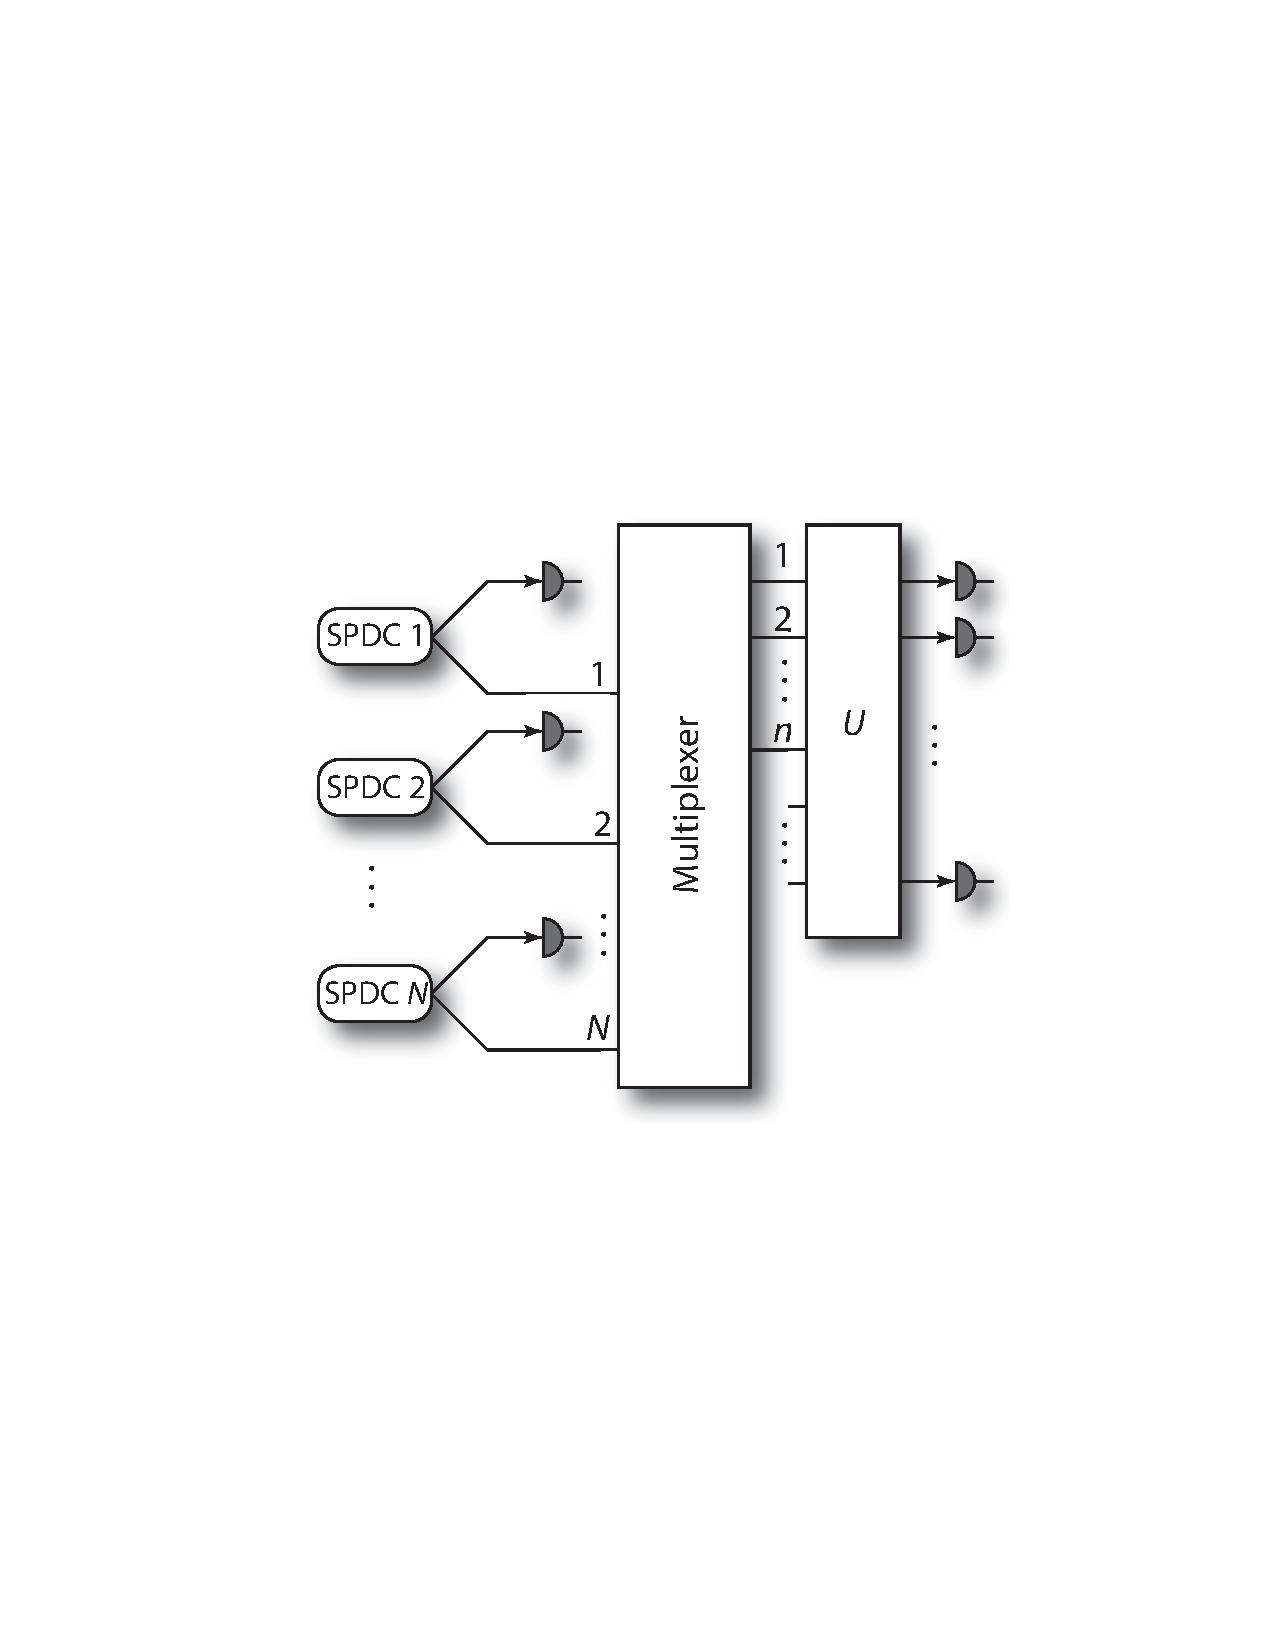
\includegraphics[width=0.7\columnwidth]{multiplexing}
\caption{Boson-sampling architecture using SPDC sources with an active multiplexer. $N$ sources operate in parallel, each heralded by an inefficient single-photon number-resolving detector. It is assumed that \mbox{$N\gg n$}, which guarantees that at least $n$ photons will be heralded. The multiplexer dynamically routes the successfully heralded modes to the first $n$ modes of the unitary network $U$. Finally, photodetection is performed and the output is post-selected on the detection on all $n$ photons.}
\label{fig:multiplexing}
\end{figure}

Another problem is that SPDC sources is that there is uncertainty in the temporal distribution of the photons. If you build a boson-sampling device using multiple SPDC sources it is extremely difficult to temporally align each of the $n$ photons going into the device. The error term associated with this also scales exponentially with $n$. Exponentially scaling errors totally renders your boson-sampling device useless since we can only tolerate polynomial error scaling with $n$. 

\subsection{Linear optical networks (Keith)}
After the input state has been prepared it then passes through some linear optical network denoted by $U$. $U$ transforms the input state and may be completely characterized before the experiment using coherent state inputs \cite{bib:PhysRevLett.73.58}. This network is composed of an array of discrete elements, namely, beam-splitters and phase shifters.  A beamsplitter and phase shifter can be combined and represented in the following general form \cite{bib:GerryKnight05},
\begin{equation} \label{eq:BS}
U_{\mathrm{BS}}(t) = \left[ \begin{array}{cc}
e^{i(\alpha-\frac{\beta}{2}-\frac{\gamma}{2})}\mathrm{cos}\left(\frac{\delta}{2}\right) & -e^{i(\alpha-\frac{\beta}{2}+\frac{\gamma}{2})}\mathrm{sin}\left(\frac{\delta}{2}\right)  \\
e^{i(\alpha+\frac{\beta}{2}-\frac{\gamma}{2})}\mathrm{sin}\left(\frac{\delta}{2}\right) & e^{i(\alpha+\frac{\beta}{2}+\frac{\gamma}{2})}\mathrm{cos}\left(\frac{\delta}{2}\right)
\end{array} \right], 
\end{equation}
where $0\leq\alpha\leq2\pi$ and $0\leq\{\beta,\gamma,\delta\}\leq\pi$ are arbitrary phases. It was shown by Reck \emph{et al.} that an arbitrary unitary transformation $U$ can be constructed with  $O(m^2)$ optical elements \cite{bib:PhysRevLett.73.58}, where $m$ is the number of inputs to the boson-sampling device. It would seem as though hundreds of optical elements would need to be aligned which would also occupy entire optical laboratories. This is quite impracticable and is a problem with boson-sampling. There are other options to get around some of these troubles.  

One method to simplify the linear optical network is to use integrated waveguides. Quantum interference was first demonstrated in this technology by Peruzzo \emph{et al.}\cite{bib:peruzzo2011multimode}. This technology integrates the beam-splitters and phase shifters into a 

A major experimental problem with creating a unitary $U$ is aligning $O(m^2)$ optical elements. A potential route around this is to use time-bin encoding in a loop based architecture \cite{bib:motes2014scalable}. The major advantage of this architecture is that it only requires two delay loops, two on/ off switches, and one controllable phase shifter as shown in Fig. \ref{fig:fiber_loop}, thus the aligning problem is eliminated. A major problem with this architecture however is that it remains difficult to dynamically control a phase-shifter with high fidelity. 

\begin{figure}[!htb]
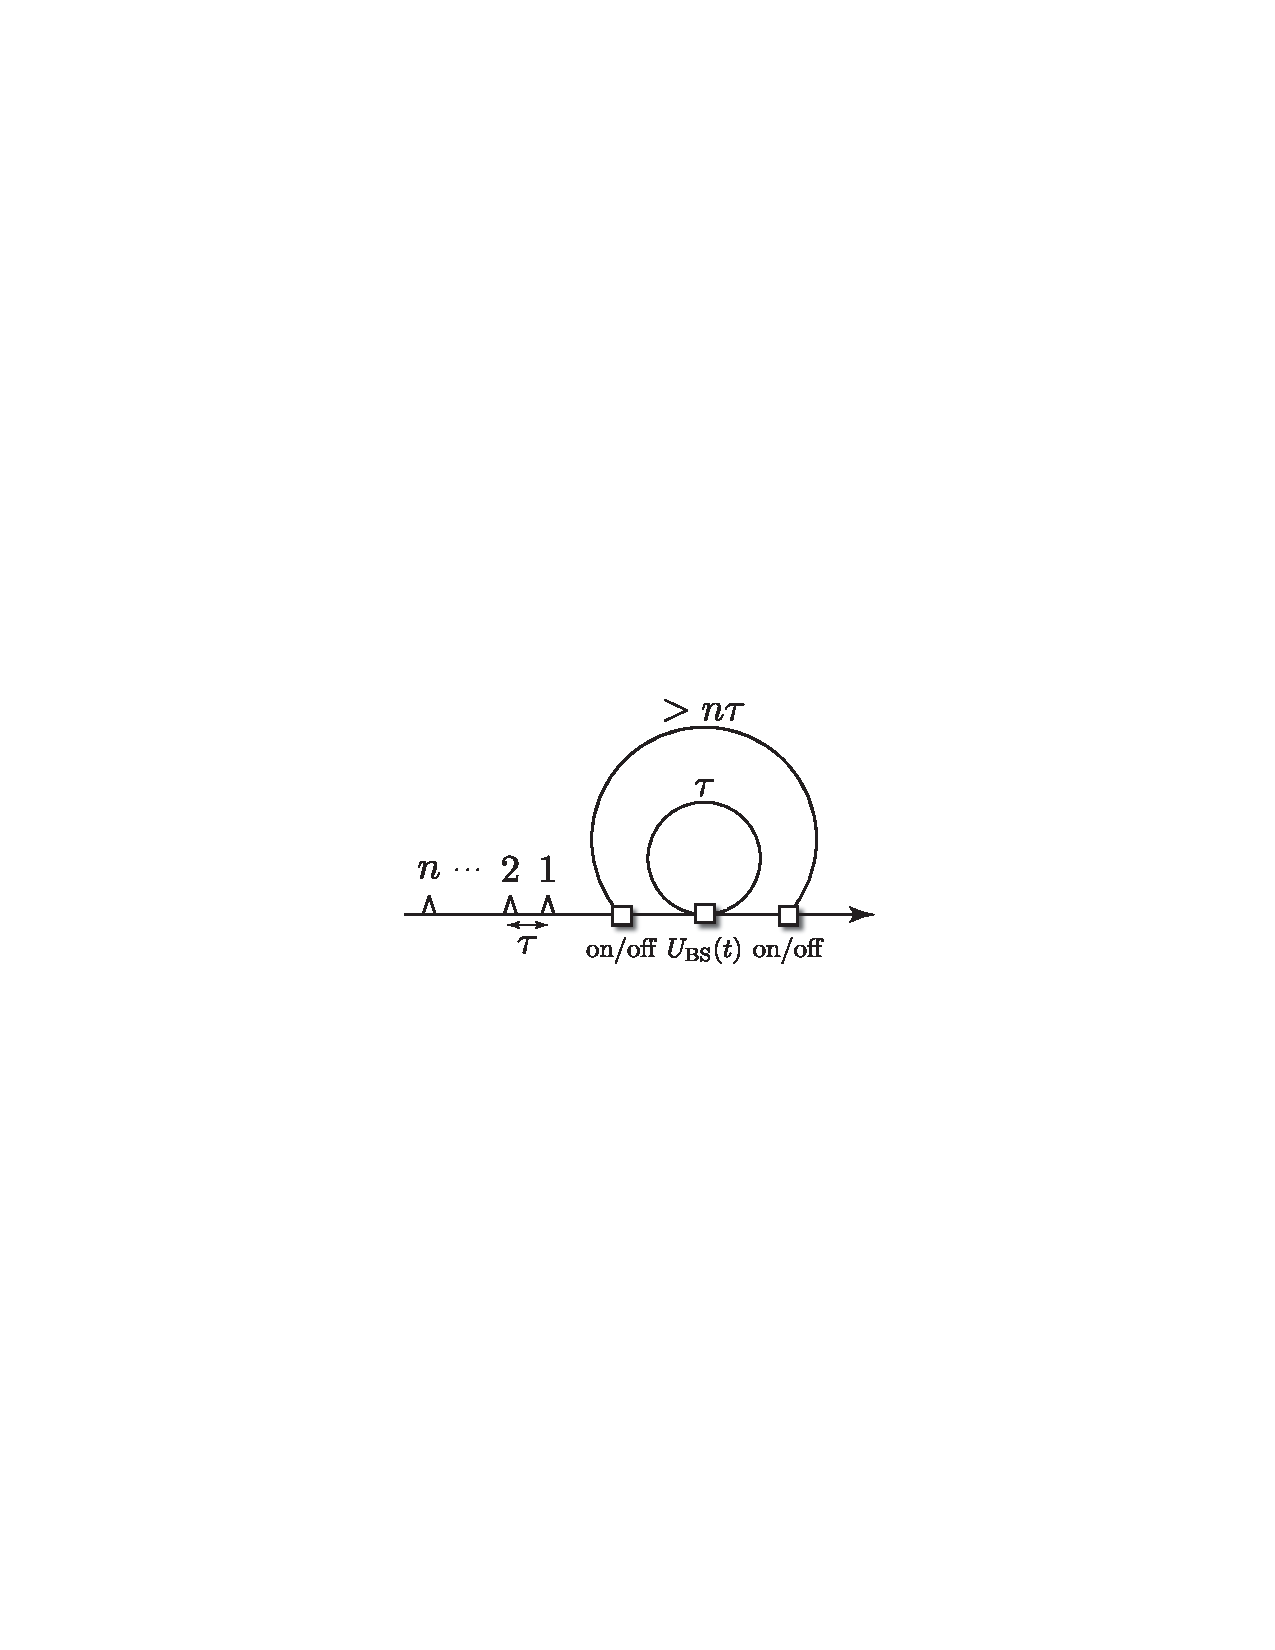
\includegraphics[width=0.7\columnwidth]{fiber_loop}
\caption{The full time-bin encoding architecture for implementing a boson-sampling device. Single photons arrive in time-bins instead of in spatial modes. Each time-bin corresponds to spatial modes in the boson-sampling scheme and are separated by time $\tau$. The photon train gets coupled completely in by the first switch. The photons then transverse the inner loop such that each time-bin may interact. The first (last) photon is coupled completely in (out) so that input and output time-bins match. The outer loop allows an arbitrary number of the smaller loops to be applied consecutively which is determined by the third switch. Finally, the photon train is measured at the output and regular boson-sampling statistics apply. Note that any delay line will work in this architecture.}
\label{fig:fiber_loop}
\end{figure}

\begin{itemize}
\item Reck et al.
\item Waveguides; cite Alberto Peruzzo
\item Discrete elements; beam-splitters and phase shifters; give general equation of beam-splitter from Knight book.
\item in case of other types of bosons it need to be optical.
\item alignment.
\item be sure to describe issues to overcome
\end{itemize}

\subsection{Photo-detection (Keith)}

\begin{itemize}
\item List different types of detectors
\item don't need to be number resolving.
\item be sure to describe issues to overcome
\end{itemize}

\section{Conclusion (Jon)}

%
% Acknowledgments
%

\begin{acknowledgments}
This research was conducted by the Australian Research Council Centre of Excellence for Engineered Quantum Systems (Project number CE110001013).
\end{acknowledgments}

%
% Bibliography
%

\bibliography{bibliography}

\end{document}
